\section{ Web-Programmierschnittstelle (Web-API)}
% Einleitung, Motivation
Die Webseite der Wetterstation bietet den interessierten Personen Informationen zum aktuellen Wetter in Arbon. Diese Informationen sind aber nicht nur für Menschen interessant, sondern auch für andere Computer beziehungsweise Server. Das Seebad Arbon zum Beispiel möchte die Wassertemperatur der Wetterstation auf ihrer Webseite anzeigen. Um die Kommunikation von Server zu Server zu vereinfachen werden maschinenlesbare Schnittstellen eingesetzt, sogenannte application programming interfaces (API). Abbildung\,\ref{img:humanvsmachine} zeigt den Unterschied der beiden Darstellungsarten. Auf der linken Seite ist die für den Menschen grafisch mit Farben und Formen aufbereitete Information der Lufttemperatur, auf der rechten Seite die schlichte und rein textbasierte Maschinenversion.

\begin{figure}[htbp!]
  \fbox{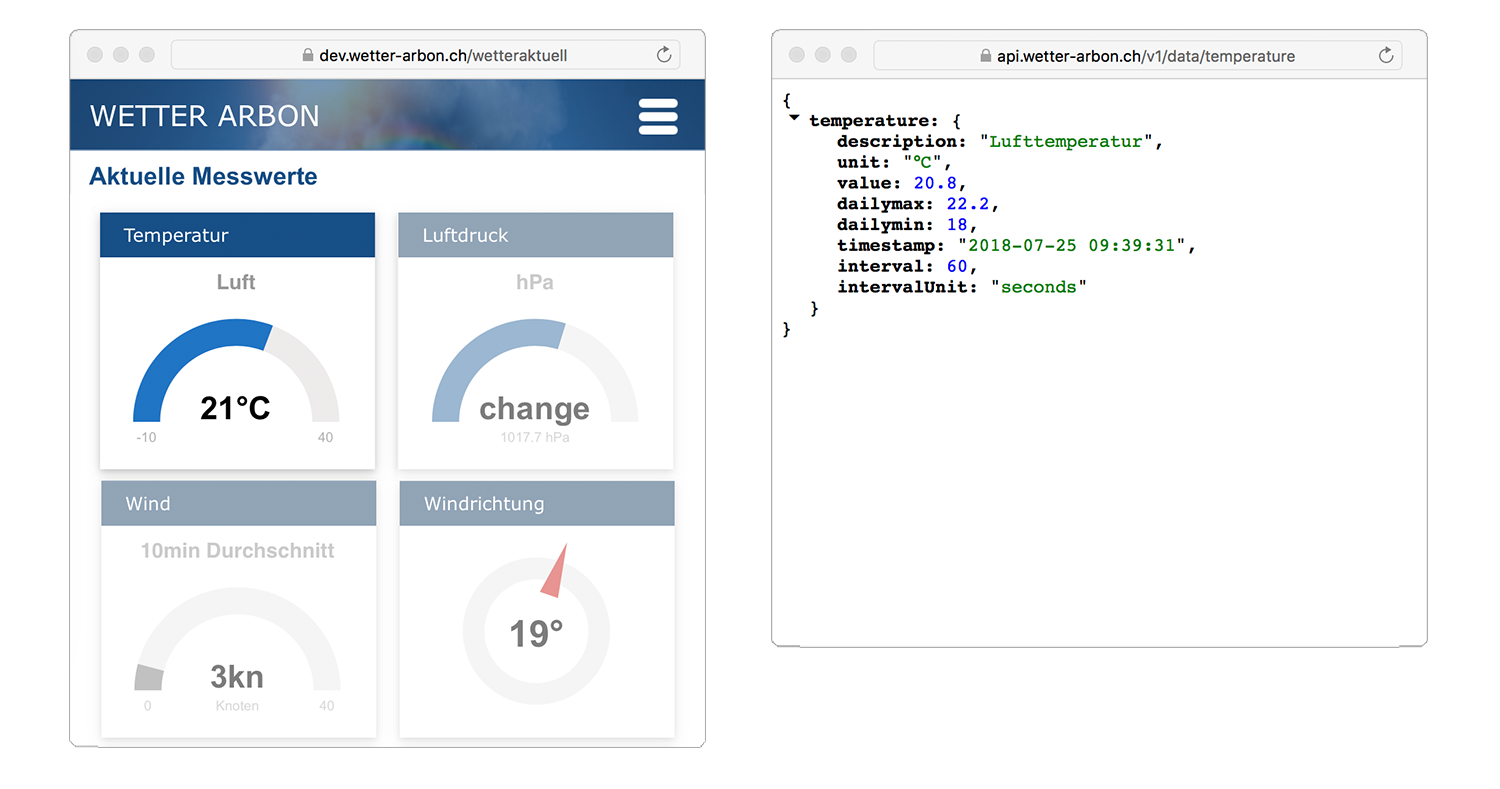
\includegraphics[width=\textwidth-2\fboxsep-2\fboxrule]{img/humanvsmachine}}
	\centering
	\caption{Grafische (HTML) versus maschinenlesbare (JSON) Darstellung}
	\label{img:humanvsmachine}
\end{figure}

%% ############################################################################
%% Unterkapitel
%% ############################################################################
\subsection{Konzipierung und Design der API}
Die Wetterstation liefert unterschiedliche Arten von Informationen, dies sind etwa Temperaturdaten, den Status der Sturmwarnung und eine Verlinkung zur Webcam. Die API wurde deshalb in drei Kategorien aufgeteilt:

\begin{itemize*}
\item Messdaten (data)
\item Zusatzinformationen (misc)
\item Webcam-Links (webcam)
\end{itemize*}

\noindent
\emph{Data} ist für die direkten bzw. indirekten Messdaten der Wetterstation vorgesehen. Unter \emph{misc} werden verschiedene Arten von Daten, welche von Dritten abgegriffen werden, verarbeitet, wie zum Beispiel der Status der Sturmwarnung. Unter \emph{webcam} werden Links für die Webcam zur Verfügung gestellt. Unterhalb der Kategorien befinden sich die Informationseinheiten. Es handelt sich hierbei um in sich geschlossene Datenblöcke, wie in Abbildung\,\ref{img:humanvsmachine} rechts dargestellt. Die komplette Struktur mit allen möglichen Abfragen ist in Abbildung\,\ref{img:hierarchie} dargestellt.

Die Struktur wurde so gewählt, dass sie logisch ist, sich beliebig erweitern lässt und die URL trotzdem möglichst kurz ist. Denn der API-Aufruf, das heisst die URL entspricht genau dieser hierarchischen Datenstruktur. Um zum Beispiel die aktuellen Lufttemperatur zu erhalten muss folgende URL verwendet werden: \url{https://api.wetter-arbon.ch/v1/data/temperature}. Wenn mehrere Werte auf einmal abgefragt werden sollen, kann die URL eine oder zwei Stufen höher aufgerufen werden also zum Beispiel \url{https://api.wetter-arbon.ch/v1/data/} beziehungsweise \url{https://api.wetter-arbon.ch/v1/}. In diesem Fall werden jeweils alle Daten unterhalb der gewählten Hierarchiestufe ausgegeben.


\begin{figure}[htbp!]
  \fbox{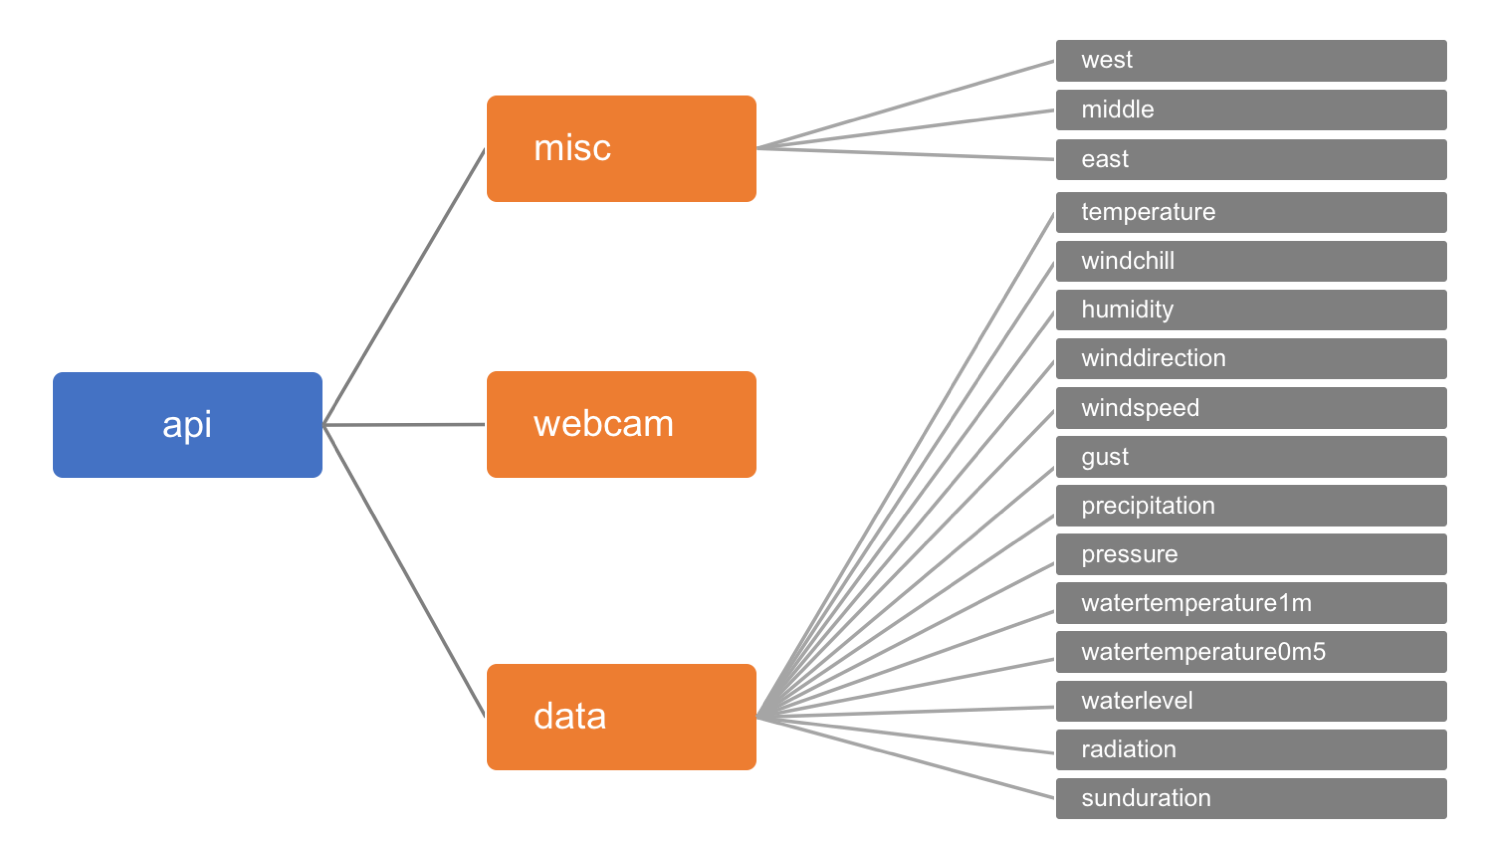
\includegraphics[width=\textwidth-2\fboxsep-2\fboxrule]{img/hierarchie}}
	\centering
	\caption{Die dreistufige Datenhierarchie der API}
	\label{img:hierarchie}
\end{figure}


% DE oder EN?


\subsubsection{Anwendung des REST-Prinzips}
Heutzutage werden viele API nach dem REST-Prinzip\,\footnote{REST: Representational State Transfer} von Roy Fielding entwickelt. Der REST-Architekturstil bietet diverse Vorteile unter anderem bezüglich Skalierbarkeit und Sicherheit, wie in der \href{https://www.ics.uci.edu/~fielding/pubs/dissertation/top.htm}{Doktorarbeit}~\cite{Fielding:2000:ASD:932295} von Fielding nachzulesen ist. Eines der wichtigsten Prinzipen daraus ist die Zustandslosigkeit einer Anfrage. Das heisst jede Anfrage vom Client zum Server enthält alle notwendigen Informationen; auf dem Server muss nichts zwischengespeichert werden. REST verwendet zudem die von HTTP zur Verfügung gestellten Methoden\cite{LornaJaneMitchell2013oreilly}. Bei der Wetterstation wird nur die GET-Methode verwendet, da die API der Wetterstation sozusagen ein read-only-Dienst darstellt. Eine Server-Anfrage sieht dann zum Beispiel so aus wie in Listing\,\ref{lst:apirequest}. Bei einem POST-Aufruf wird das gleiche Resultat geliefert wie beim entsprechenden GET-Aufruf. 


\vspace{3mm}
\begin{lstlisting}[label=lst:apirequest,caption=RESTful-Serveranfrage, language=HTML5, style=php]
GET /v1/data HTTP/1.1
Host:           api.wetter-arbon.ch
Cache-Control:  no-cache
\end{lstlisting}
\vspace{3mm}


\subsubsection{Semantische Versionierung}
Versionsnummern unterscheiden einzelne Versionen einer Software, um deren Weiterentwicklungen nachvollziehbar zu kennzeichnen. Die Versionsnummer der API ist beim Aufrufen der oberste Hierarchiestufe sichtbar, siehe Listing\,\ref{lst:versionierung}. Angewendet wird dabei die semantische Versionierung\footnote{\url{https://semver.org}}. Diese teilt die Versionsnummer in folgende drei Bereiche auf: MAJOR.MINOR.PATCH, wobei die drei Bereich unterschiedliche Bedeutungen haben:

\begin{description*}
  \item[MAJOR] Neuerungen hinzugefügt; inkompatibel mit Vorversion
  \item[MINOR] Funktionen hinzugefügt; kompatibel mit Vorversion
  \item[PATCH] Fehler behoben; kompatibel mit Vorversion
\end{description*}

\vspace{3mm}
\begin{lstlisting}[label=lst:versionierung,caption=Versionierungsangabe auf der obersten Hierarchiestufe, language=HTML5, style=php]
{
v1: {
 version: "1.1.1",
 misc:   {...}
 webcam: {...}
 data:   {...}
}
\end{lstlisting}
\vspace{3mm}

\noindent
Die MAJOR-Version unterscheidet demnach zwischen verschiedenen inkompatiblen Versionen. Eine API wird häufig von einem anderen Computer das heisst von einem Programm aufgerufen. Eine inkompatible Änderung würde dazu führen, dass dieses Programm unter Umständen nicht mehr korrekt funktioniert. Aus diesem Grund wurde die MAJOR-Nummer in die URL der API aufgenommen. Auf diese Weise kann parallel eine Version 2 implementiert werden, ohne dass die Nutzer der Version 1 betroffen sind. Die URL setzt sich demnach zusammen aus: \\

\noindent
\texttt{Protokoll://Host/Versionsnummer/Endpunkt}\\
und als Beispiel:\\
\url{https://api.wetter-arbon.ch/v1/data/}

\noindent
\Diskussionspunkt{Erklärgrafik hinzufügen}


\subsubsection{Auswahl des Response-Datenformats}
Damit sich die Computer gegenseitig verstehen, ist es wichtig, dass die Kommunikation in einem standartisierten Datenformat erfolgt. Hier besteht die Möglichkeit zu wählen zwischen JSON, XML oder CSV. Es können auch andere Formate genutzt werden. Wichtig ist jedoch, dass der Server sowie der Client wissen welches Format genutzt wird. Der Server sendet deshalb im Header der Antwort die entsprechende Formatbezeichnung mit (zum Beispiel \texttt{ Content-Type: application/json}). Der Client kann im Header zwar angeben in welchem Format er die Antwort gerne hätte, der Server liefert aber unabhängig davon JSON zurück.

Als Datenformat der API wurde JSON\footnote{JSON: Javascript Object Notation} gewählt, da es sich um ein simples und im Webbereich häufig eingesetztes Datenformat handelt, welches nicht viel Speicherplatz benötigt. Nebst der Lesbarkeit für Maschinen, kann es auch von Menschen einfach gelesen werden. Javascript beispielsweise handhabt JSON nativ und auch die Verwendung in PHP ist simpel, wie im Buch PHP Web Services \cite{LornaJaneMitchell2013oreilly} erwähnt wird. Eine JSON-Antwort mit sämtlichen Werten ist in Anhang Listing \ref{lst:JsonTree} dargestellt. Bei hierarchischen Datenstrukturen spricht man auch von einem Daten-Tree.

%% ############################################################################
%% Unterkapitel
%% ############################################################################
\subsection{Back end Architektur der API}
% Rahmenbedingung: Serverseitige Programmiersprache ist eingeschränkt von Hostpoint auf .......
% Warum wurde php gewählt?
Für die API gibt es jedoch eine wichtige Bedingung. Sie muss in php geschrieben werden, da Hostpoint kein Javascript auf der Serverseite erlaubt.



\subsubsection{Auswahl des PHP-Frameworks}
% Sollte es KO-Kriterien geben, werden diese bereits im Vorfeld der Nutzwertanalyse dazu genutzt, die Alternativen für den Vergleich einzuschränken.
% KO-Kriterium: kostenlos und von Hostpoint unterstützt


% https://www.quora.com/What-is-a-PHP-framework
% https://www.quora.com/Where-can-I-learn-to-create-a-PHP-REST-API-without-using-a-framework
% https://fachinformatiker-anwendungsentwicklung.net/nutzwertanalyse-in-der-projektdokumentation/

% Nutzwertanalyse
\begin{table}[htbp!]
  \setlength\extrarowheight{3pt} % for a more "open" look
  \begin{tabularx}{\textwidth}{|>{\RaggedRight\hspace{0pt}}p{3cm}|p{2.2cm}||p{2.2cm}|X|X|X|}

  \hline
  & \bfseries Gewichtung
  & \bfseries \href{https://codeigniter.com}{CodeIgiter}
  & \bfseries \href{https://www.slimframework.com}{Slim}
  & \bfseries \href{https://lumen.laravel.com}{Lumen}
  & \bfseries ohne\\

  \hline
  \textbf{Dokumentation}
  & 4
  & 3
  & 3
  & 2
  & 3 \\

  \hline
  \textbf{Langlebigkeit}
  & 1
  & 1
  & 1
  & 2
  & 3 \\

  \hline
  \textbf{Funktions-umfang}
  & 2
  & 2
  & 2
  & 2
  & 1 \\

  \hline
  \textbf{Stabilität und Sicherheit}
  & 4
  & 2
  & 3
  & 3
  & 3 \\

  \hline
  \textbf{Footprint}
  & 1
  & 1
  & 3
  & 3
  & 3 \\

  \hline
  \hline
  \textbf{Total}
  & -
  & 9
  & 12
  & 12
  & 13 \\

  \hline
  \textbf{gewichtet}
  & -
  & 26
  & 32
  & 29
  & 32 \\

  \hline
  \end{tabularx}
  \caption{Nutzwertanalyse der evaluierten php-Frameworks}
  \label{table:php-framework} % label muss NACH caption stehen!!!!
\end{table}


\paragraph*{Kriterien für die Auswahl}
Folgende Kriterien für die Auswahl des php-Frameworks wurden berücksichtigt:
\begin{itemize*}
\item Dokumentation und Einarbeitungszeit: Sind die Funktionen zentral und verständlich dokumentiert?
\item Langlebigkeit: Läuft das Framework auch unter neuen PHP-Versionen?
\item Funktionsumfang: Bietet das Framework Features, die ein produktives Entwickeln ermöglichen (Routing, Header, Response-Formatierung)?
\item Stabilität und Sicherheit: Werden regelmässig Updates zur Verfügung gestellt?
\item Footprint: Ist die Dateigrösse in einem verhältnismässigen Rahmen?
\end{itemize*}




\paragraph*{Gewichtung der Kriterien}
% Gewichtung wird vor der Durchführung des eigentlichen Vergleichs festgelegt
% Gewichtung der Kriterien muss in der Projektdokumentation begründet werden
Die Gewichtungsskala für die Kriterien reicht von 1 (weniger wichtig) bis 4 (sehr wichtig). Für die Auswahl des php-Frameworks wurde folgende Gewichtung vorgenommen:

\begin{itemize*}

\item 4 Dokumentation: Da es sich um das Abschlussprojekt des Autors mit fester Zeitvorgabe handelt, ist besonders wichtig, dass die Sprache ihm bereits bekannt ist. Des Weiteren muss auch die Interessensgemeinschaft die API in einem vernüftigem Zeitrahmen Unterhalten können.

\item 1 Langlebigkeit: Da es sich um eine Webanwendung handelt, die wahrscheinlich häufig an neue Möglichkeiten angepasst werden muss, ist die Langlebigkeit von geringerer Wichtigkeit.

\item 2 Funktionsumfang: Gerade im Webumfeld setzt das Unternehmen auf neue Technologien und möchte neue Entwicklungen zeitnah einsetzen.

\item 4 Stabilität und Sicherheit: Da die Arbeit anschliessend öffentlich ist und gewährleistet werden muss, dass die Webseite funktionsfähig ist.

\item 1 Footprint: Da für die Webseite genügend Speicherplatz vorhanden ist. Ist der Footprint nich sehr wichtig.



\end{itemize*}




\paragraph*{Bewertungsskala für die Kriterien}
% Skala mit erlaubten Punktwerten und exakte Begründung für die vergebene Punktzahl
% kleine Skala verwenden z.B. 1 bis 3, und definiert exakt, wann welcher Wert vergeben wird.
% unbedingt angegeben, welche Werte gut und welche schlecht sind

Als mögliche Werte für die genannten Kriterien werden die Zahlen 1 (schlecht) bis 3 (gut) verwendet. Im Folgenden wird festgelegt, wann welcher Wert bei den einzelnen Kriterien vergeben wird.

\begin{itemize*}
\item Dokumentation und Einarbeitungszeit
  \begin{enumerate*}
  \item Keine zentrale Dokumentation vorhanden
  \item Zentrale Dokumentation vorhanden, wenig ausführlich
  \item Zentrale Dokumentation vorhanden, ausführlich und verständlich
  \end{enumerate*}
\item Langlebigkeit
  \begin{enumerate*}
  \item Keine Angabe, ob die neue PHP-Version (7.2) unterstützt wird
  \item Neue PHP-Version (7.2) wird unterstützt
  \item Neue PHP-Version werden durch regelmässige Updates unterstützt
  \end{enumerate*}
\item Funktionsumfang
  \begin{enumerate*}
  \item Keine zusätzlichen Funktionen verfügbar
  \item Routineaufgaben sind als Funktionen verfügbar
  \item Routineaufgaben sind als Funktionen verfügbar
  \end{enumerate*}
\item Stabilität und Sicherheit
  \begin{enumerate*}
  \item Wenig verwendet bzw. getestet
  \item Vielverwendet, selten Updates
  \item Vielverwendet mit regelmässigen Updates
  \end{enumerate*}
\item Footprint
  \begin{enumerate*}
  \item Grösser als 5MB
  \item Zwischen 1...5MB
  \item Kleiner als 1MB
  \end{enumerate*}
\end{itemize*}


\paragraph*{Entscheidung um kein Framework zu nehmen}
% Nutzwert: stellt das Endergebnis der Nutzwertanalyse dar und repräsentiert die kumulierten bewerteten Kriterien der einzelnen Alternativen.
% Letztlich müssen alle Koeffizienten mit denen der anderen Alternativen verglichen werden, um den Gewinner zu bestimmen
% der einzelne Nutzwert ist nicht aussagekräftig, sondern muss immer ins Verhältnis zu den anderen Ergebnissen gesetzt werden
Wie das Resultat aus der Nutzwertanalyse (Tabelle \ref{table:php-framework}) aufzeigt, bleiben zwei Möglichkeiten übrig. Zum einen das Slim-Framework, zum anderen kein Framework zu nehmen. Bei der Dokumentation schneidet beides gleich ab. Denn wird kein Framework benutzt, kann die PHP-Dokumentation zu Handen genommen werden. Jedoch bestehen grosse Unterschiede bei der Langlebigkeit. Hier kann ohne Framework auf die standard Funktionen zurückgegriffen werden. Ein weiterer Vorteil ist, dass man hier die Kontrolle über den Code hat. So können Versionsspezifische Funktionen schnell angepasst werden, ohne das weiterer Code geändert werden muss. Beim Funktionsumfang schneidet das Framework besser ab. Konkret heisst dies, dass einzelne Funktionen schon vorgegeben sind und dem jeweiligen Nutzen nur angepasst werden muss. Das ist der Nachteil wenn ohne Framework gearbeitet wird. Hier muss jede Funktion selber codiert werden.\\
Bei der Stabilität und Sicherheit schneiden beide gleich ab. Dies hängt jedch, wenn ohne Framework gearbeitet wird, vorallem auch vom Programmierer und deren Tests ab. Beim Footprint sind beide gleichauf. Beide benötigen weniger als 5 Mb.\\
Der Ausschlaggebende Punkt in dieser Arbeit ohne Framework zu arbeiten ist die Grösse der API, sowie den Wunsch der IG Arbon, die ganze Arbeit so zu gestalten, dass praktisch kein Unterhalt notwendig ist. Bei der API wurde deswegen darauf geachtet schon alles mit den Funktionen aus PHP 7 zu gestalten. Weiter ist die API so zu gestaltet, wo möglich, auf Versionsspezifische Funktionen zu verzichten. 



\subsubsection{Bottom up - Funktionsprinzip}
Serverseitig wurde die API aus hierarchischer Sicht von unten nach oben entwickelt. Das heisst die Abfrage auf die Informationseinheit bildet den Kern der API. Die Abfrage einer Informationseinheit ist in Abbildung\,\ref{img:APIFiles} schematisch dargestellt. Die GET-Anfrage des Browsers wird als erstes dem PATH-File übergeben. Dort wird der Endpunkt das heisst die gewünschte Informationseinheit über einen Switch-case, wie in Listing\,\ref{lst:switchCase} dargestellt, ermittelt. Danach wird ein assoziatives Array (siehe Abbilung\,\ref{img:assozArray}) erstellt, welches alle nötigen Parameter enthält, sodass im createJson-File die Datenbank-Abfrage getätigt werden kann. Schlussendlich werden die Werte aus der Datenbank ins Array geschrieben und dieses in ein JSON umgewandelt und zurückgegeben. Je nach Informationseinheit gibt es Unterschiede beim Aufbau des JSONs. Für einige Messwerte sind Maximal- und Minimalwerte gewünscht. Andere Messwerte hingegen werden in verschiedene Einheiten umgerechnet (Knoten, km/h, Beaufort), damit alle Benutzer die Messwerte auch interpretieren können.

\begin{figure}[htbp!]
  \fbox{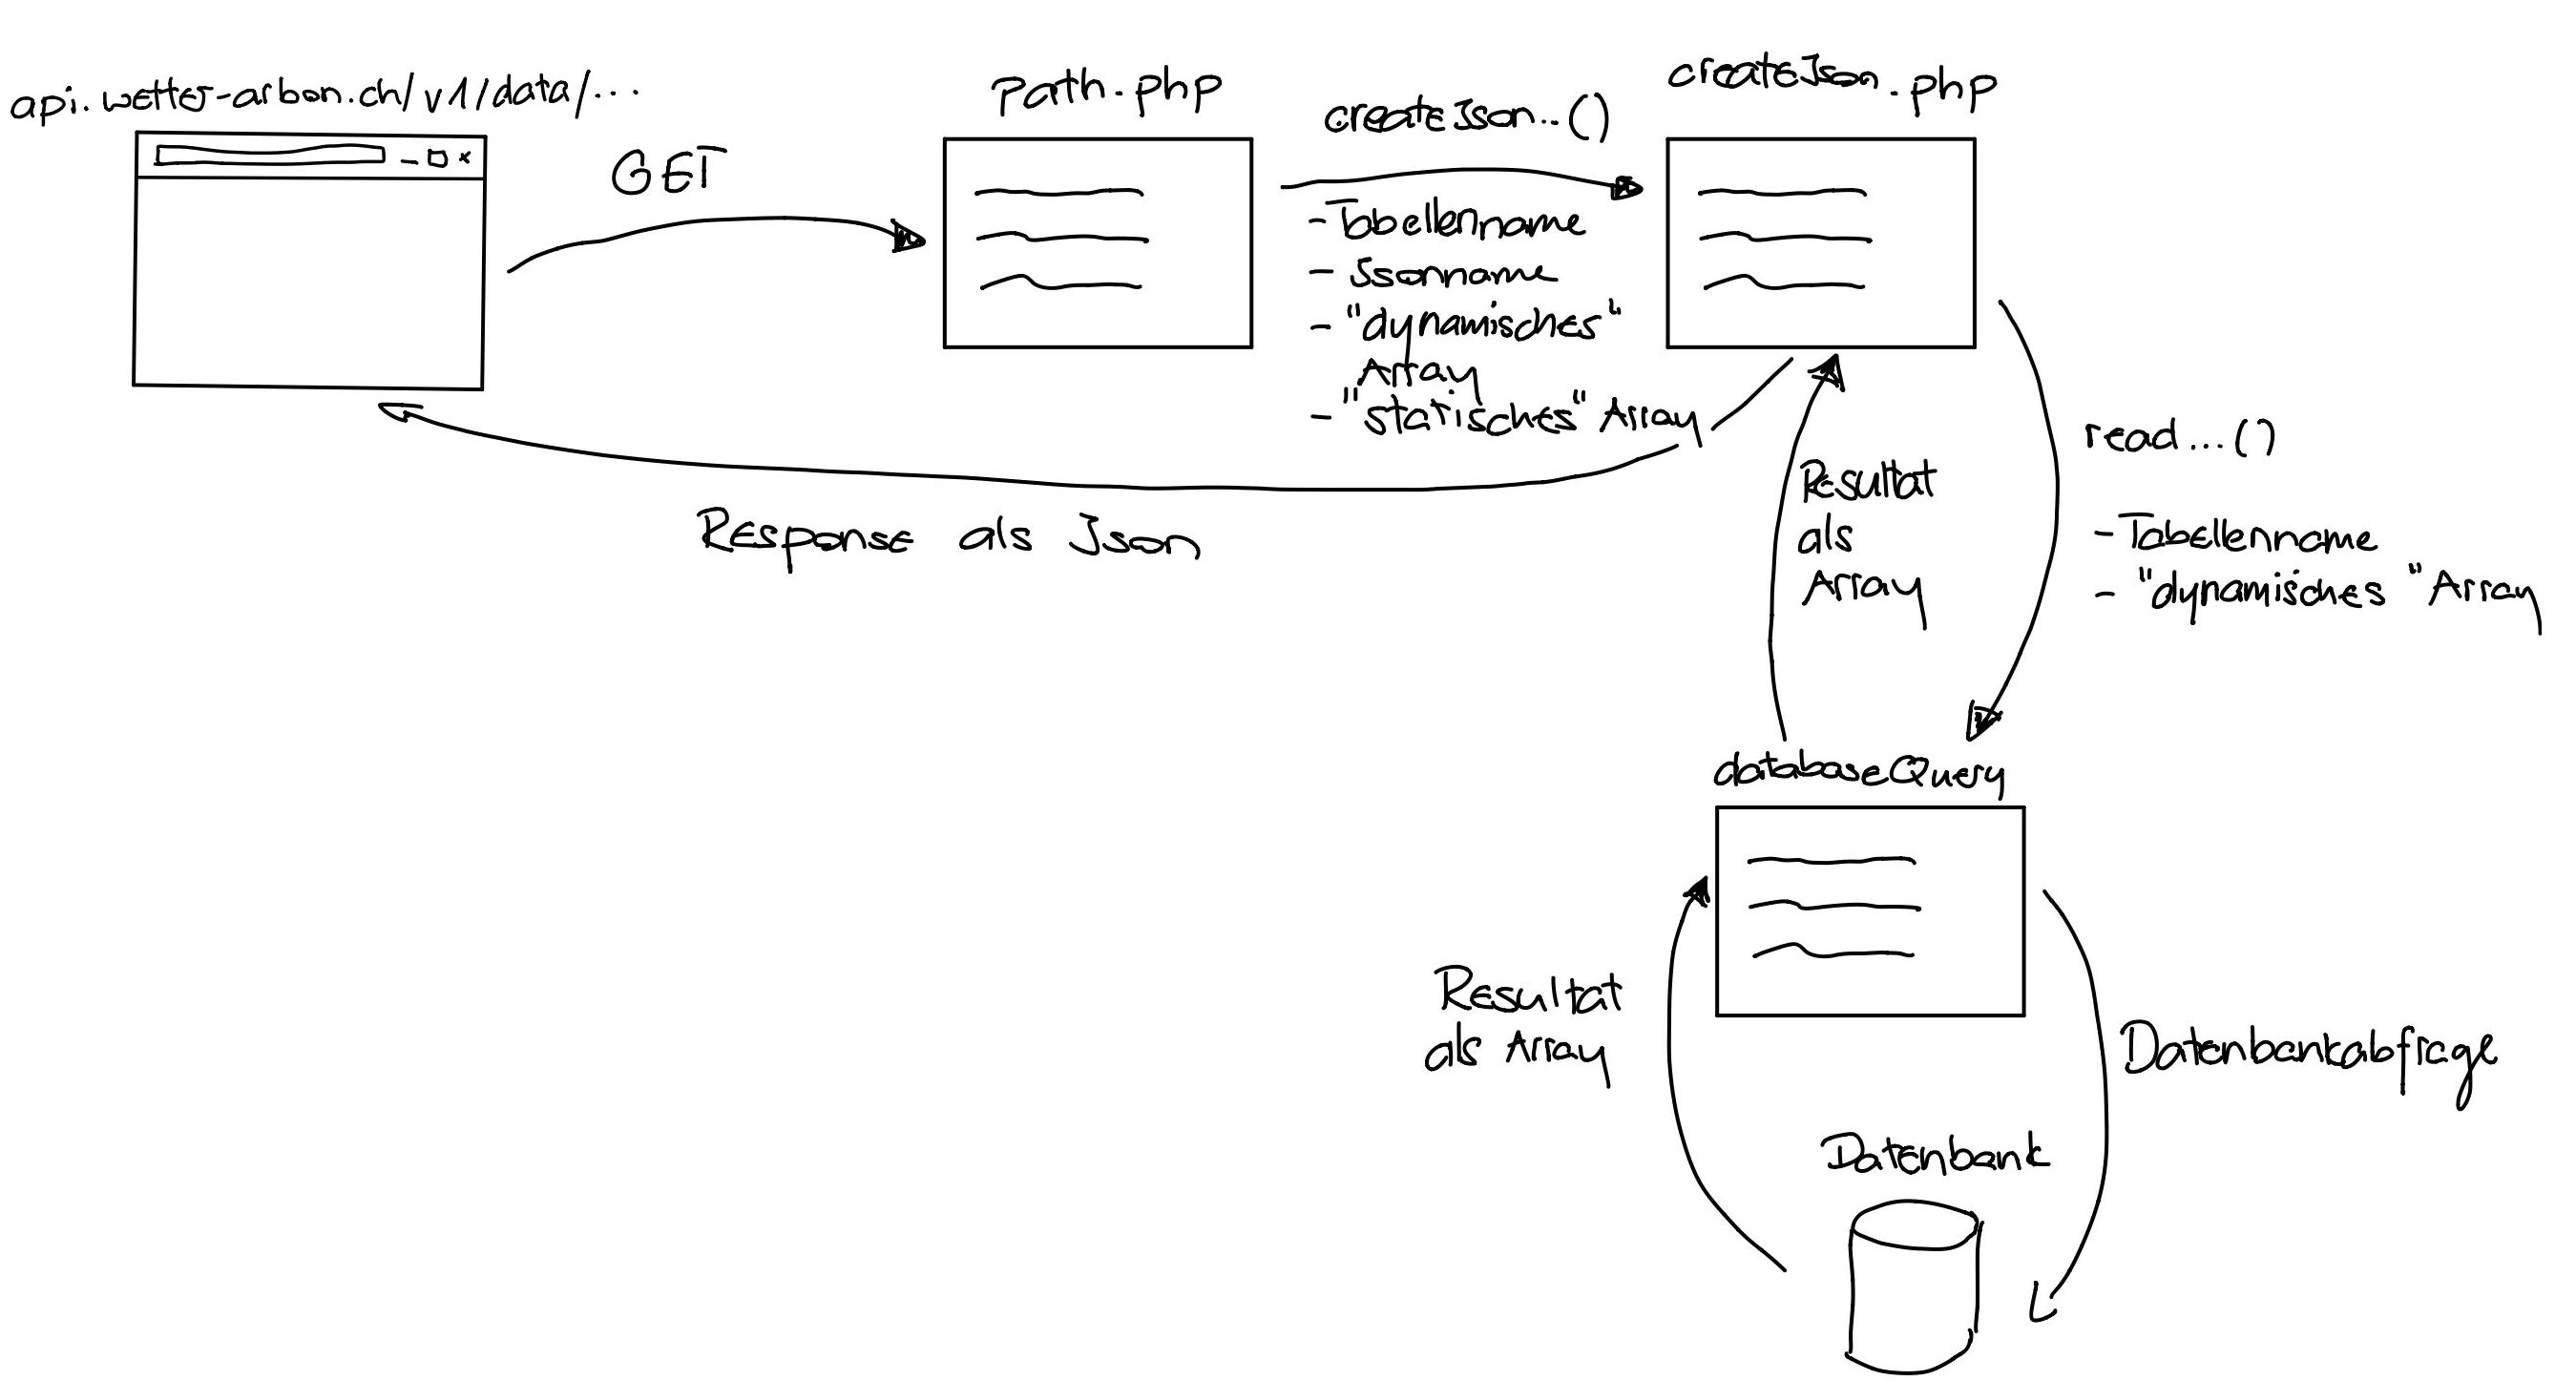
\includegraphics[width=\textwidth-2\fboxsep-2\fboxrule]{img/API_GET.jpg}}
	\centering
	\caption{Ablauf einer API GET-Abfrage auf Stufe Informationseinheit}
	\label{img:APIFiles}
\end{figure}


% Switch-Case
\vspace{3mm}
\begin{lstlisting}[label=lst:switchCase,caption=Routing innerhalb einer Kategorie mittels Switch-case, language=php, style=php]
// Beispiel: https://api.wetter-arbon.ch/v1/data/temperature
switch ($url){
 case "/v1/data/temperature":
  createJson(...); break;
 case "/v1/data/windchill":
  createJson(...); break;
 //usw.
\end{lstlisting}
\vspace{3mm}


\begin{figure}[htbp!]
  \fbox{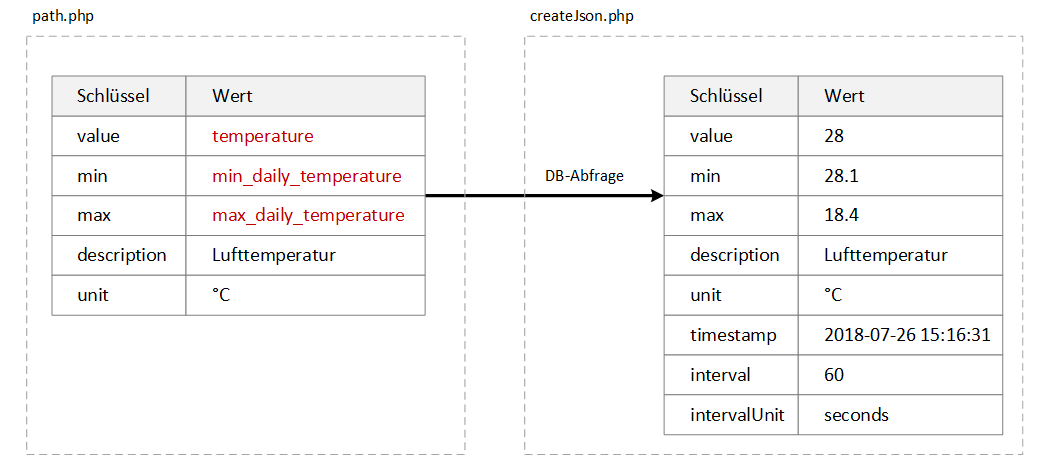
\includegraphics[width=\textwidth-2\fboxsep-2\fboxrule]{img/assozArray}}
	\centering
	\caption{Beispiel des assoziativen Arrays vor und nach der DB-Abfrage}
	\label{img:assozArray}
\end{figure}


\noindent

Die Dateistruktur wurde nach dem MVC-Prinzip nachempfunden. Das MVC-Prinzip bedeutet nichts anderes, als das drei verschiedene Dateifunktionen bestehen. Die View, path-File, sendet eine Anfrage an den Controller, createJson File. Dieser entscheidet dann was alles benötigt wird und fragt dies beim Modell an. Das Modell, databaseQuery-File, verarbeitet die angefragten Daten und sendet das Resultat zurück an den Controller. Dieser Leitet dann die Daten, in diesem Fall direkt an den Client weiter.


\subsubsection{Skalierbarkeit durch modularen Aufbau}
Die ganze API ist Modular aufgebaut, so dass sie für weitere Anwendungen oder Messwerte ausgebaut werden kann. Die Datenabfrage findet immer auf Stufe Informationseinheit statt. Findet die Abfrage auf einer höheren Stufe statt, so und werden die Informationseinheiten einzeln über eine GET-Abfrage aufgerufen (analog Abbildung\,\ref{img:APIFiles}) und anschlissend zusammengefasst. Konkret heisst dies, dass wenn zum Beispiel die URL \texttt{../v1/data} aufgerufen wird, sämtliche unter data befindenden Informationseinheiten in einer foreach-Schlaufe abgefragt, und anschlissend in einem JSON zusammengefasst werden, wie in Listing\,\ref{lst:foreach} dargestellt.

\vspace{3mm}
\begin{lstlisting}[label=lst:foreach,caption=API-Abfrage auf Stufe Kategorie, language=php, style=php]
$url=array(
  "/v1/data/temperature",
  "/v1/data/windchill",
  "/v1/data/humidity",
  "/v1/data/winddirection",
  "/v1/data/windspeed",
  "/v1/data/gust",
  "/v1/data/precipitation",
  "/v1/data/pressure",
  "/v1/data/weathericon",
  "/v1/data/forecasticon",
  "/v1/data/watertemperature1m",
  "/v1/data/watertemperature0m5",
  "/v1/data/waterlevel",
  "/v1/data/radiation",
  "/v1/data/sunduration"
);

foreach($url as $url){
  $json = file_get_contents('https://api.wetter-arbon.ch'.$url);
  $obj = json_decode($json,true);
  $jsonArray = array_merge_recursive($jsonArray, $obj);
}
\end{lstlisting}
\vspace{3mm}



%% ############################################################################
%% Unterkapitel
%% ############################################################################
\subsection{Dokumentation der API}
Die API wurde in Postman\footnote{\url{https://www.getpostman.com}} dokumentiert und ist über die Webseite\footnote{\url{https://documenter.getpostman.com/view/4035921/api-wetter-arbon/RW1XMhBK}} zugänglich. Dabei werden sämtliche Endpunkte, die von der API zur Verfügung gestellt werden aufgelistet und erklärt. Zudem werden parallel dazu die passenden Befehle dargestellt um zum Beispiel über Javascript oder PHP die API aufzurufen (rechts dargestellt in Abbildung\,\ref{img:postman}). Die Doku-Seite wird automatisch aufgerufen wenn sich in der URL-Anfrage auf \texttt{api.wetter-arbon.ch} ein Fehler befindet.

\begin{figure}[htbp!]
  \fbox{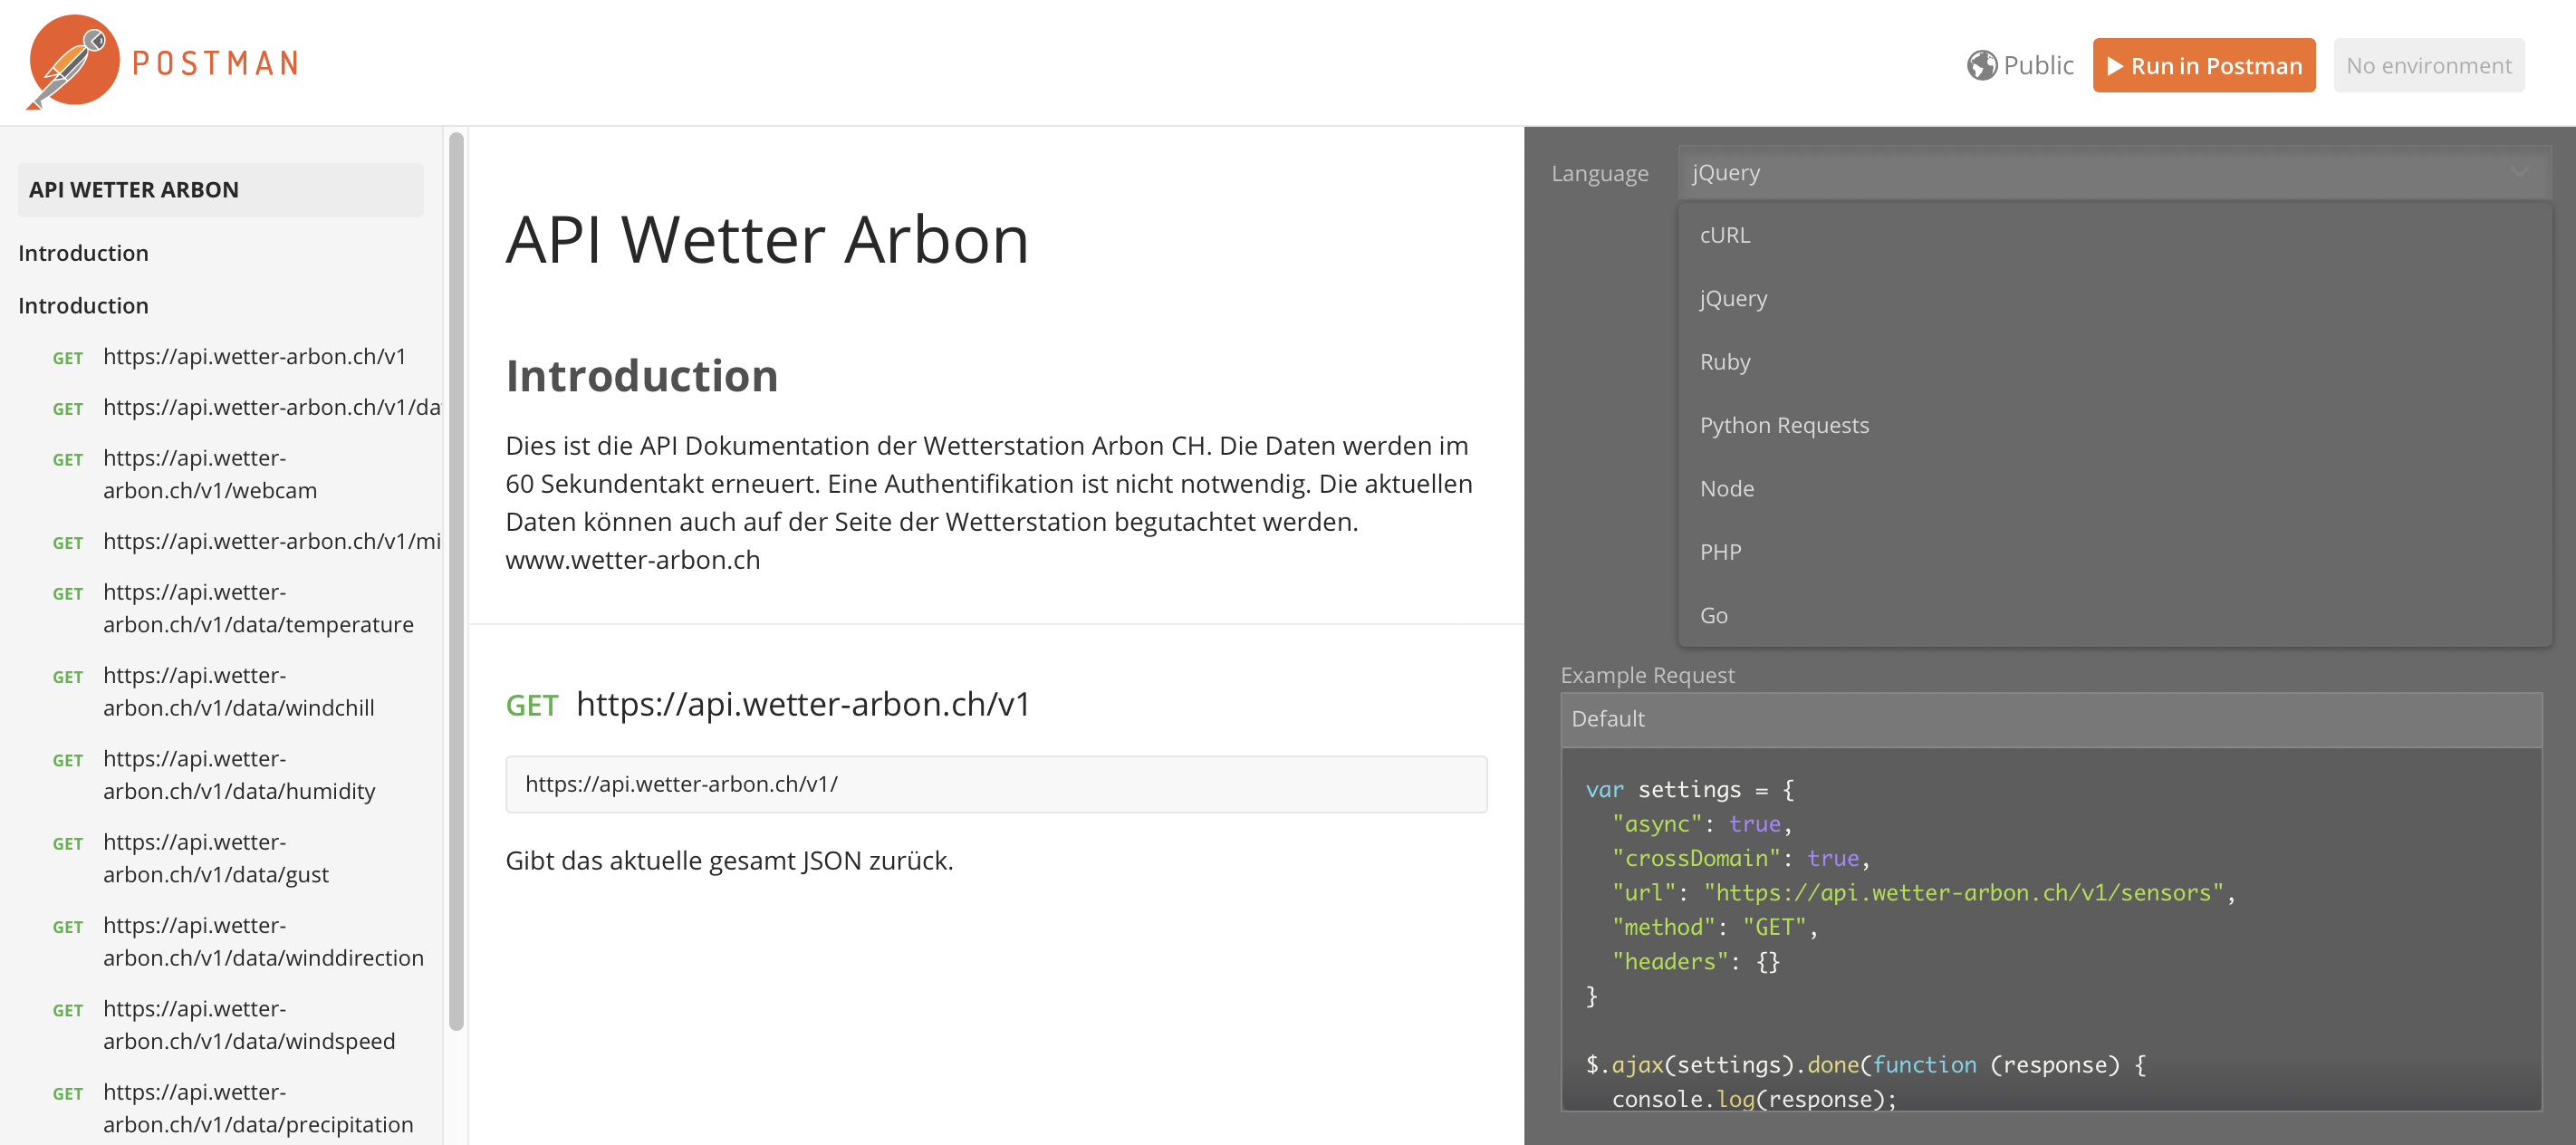
\includegraphics[width=\textwidth-2\fboxsep-2\fboxrule]{img/postman}}
	\centering
	\caption{API-Dokumentation in Postman}
	\label{img:postman}
\end{figure}

